\section{2-Way Join Example}
Correlating features across separate datasets first requires joining these datasets. Correlation coefficients ($r$) between different admissions benchmarking methods and CSC1015F course results are calculated according to the inner join shown in Equation \ref{eq:2-way-join}. A single studen number may appear multiple times in the grades data if a student repeated a course, but should appear only once on the admissions data for the first time they registered at UCT. Rows for student numbers found in the admissions data but not the grades data are not used, neither are rows found for students in the grades data but not the admissions data.

\subsection{ETL}
Using nETL, rows are extracted from the two CSV files (\textit{Admissions (2014 - 2016).csv} and \textit{Grades (2014 - 2016).csv}) independently of each other and concurrently, in batches of 5 000 and 10 000 rows respectively.

Via nETL configuration, rows from the admissions data are selected for students that are South African citizens or permanents residents, and that are undergraduates. Rows from the grades data are selected for students that attended CSC1015F during their undergraduate career. Since the admissions data doesn't have a field for course year, a natural join with grades on the \textit{anonIDnew} field is performed via nETL ($admissions \bowtie grades$) to retrieve a list of students that attended CSC1015F. Usng this list, students are selected from admissions data that attended CSC1015F.

Rows retrieved from the CSVs contain numerous fields that are not required, and so nETL is configured to apply an attribute-whitelisting process to both admissions and grade data. Batches of objects are serialized to JSON strings and loaded into a single CouchDB database via the \textit{\_bulk\_docs} endpoint. An example of a row from grade data serialized to a JSON string and as loaded into CouchDB is shown in Figure \ref{fig-json-grade}.

\begin{figure}[H]
    \centering
    \begin{mdframed}
        \centering
        \begin{minted}{text}
{
    "_id": "7530f4eed7e6bc3ef0d99a53be8ba9a2",
    "_rev": "8-232d0cf39728d41b4c5935f12469209d",
    "RegAcadYear": 2016,
    "anonIDnew": 1,
    "Course": "CSC1015F",
    "Percent": "55",
    "type_": "grade"
}    
        \end{minted}
    \end{mdframed}
    \caption[Serialized grades document]{\textbf{Figure \ref{fig-json-grade}: Serialized grades document}}
    \label{fig-json-grade}
\end{figure}

\subsection{Index Calculation}
Following loading the data from the CSVs into CouchDB, a Map function is used to produce an index of the CouchDB documents ordered by Student ID, with the guarantee that for every unique student id documents are ordered by type; the demographic document precedes the Grade documents for any given student. Knowing the order of documents via the view-index allows for performing the join on data-retrieval. Only a map function is used is required (no reduce function). That is, on Map function execution the ``type\_'' attribute is checked. If the document is a line of the Grades entity, then the key [Student ID, Course, year] is emitted along with a single number for the value - the percent achieved for the course. If the document is a line of the Admissions entity, then the key [studentNumber, 0, 0] is emitted along with an ordered list of 19 values corresponding to each of the 19 different methods of benchmarking students (discussed in Chapter \ref{aggregation}). A key of [studentNumber, year] could have been used instead, since the course is always CSC1015F. But explicitly including the year in the key makes debugging easier, and also makes the code more generically applicable if other courses are to be analyzed.

Normalization of the percentage fields (i.e. ``Percent'' for the Grades entity and the test results in the Benchmarks entity) is done via a nested function (a function defined within the map function) according to best-guess logic on how grade symbols correlate with percentage - the logic used for this is shown in Table \ref{ap-tbl-normalize-grades} and Table \ref{ap-tbl-normalize-admissions} in the appendix.

Because a student should only be represented by a single row in the admissions data and should only achieve a single grade per course per year, this 2-way join is achievable without using a reduce function. There is also no need to aggregate rows from either the admissions or grade data prior to joining. Logic of the map function is shown in the activity diagram in Figure \ref{fig-mapfn-correlation-grades}.

\begin{figure}[H]
    \centering
    \begin{mdframed}
        \centering
        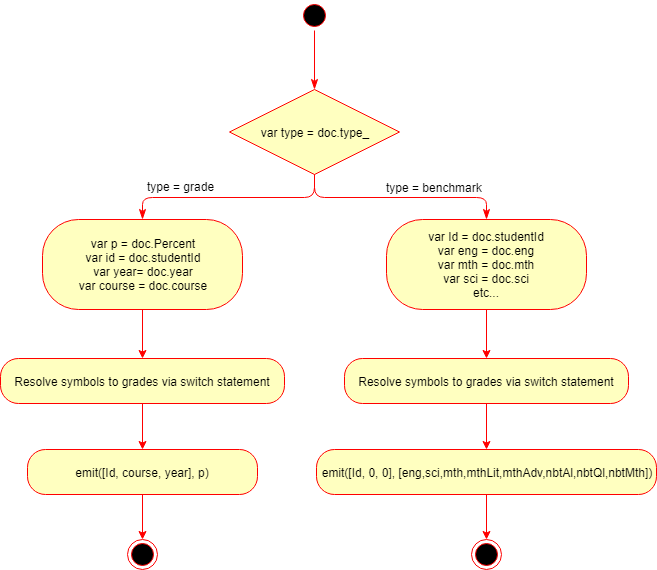
\includegraphics[scale=0.59]{./resources/figures/fig-mapfn-correlation-grades.png}
    \end{mdframed}
    \caption[\textit{Map}-function: \texorpdfstring{grades $\bowtie$ admissions}{Lg}]{\textbf{Figure \ref{fig-mapfn-correlation-grades}: \textit{Map}-function: \texorpdfstring{grades $\bowtie$ admissions}{Lg}}}
    \label{fig-mapfn-correlation-grades}
\end{figure}


\subsection{Index Retrieval}
A list function is used for data retrieval; this function scans the index iteratively (i.e. documents for each student are processed iteratively; first a student's demographic document is processed, then a student's grades documents are processed). The 2-way join is achieved in this way; for every student number the grade and admissions data is joined, and summations of various fields of the grades and each benchmark are updated. For example, for every index key:value processed the product of \mintinline{text}{CSC1015F \% x each benchmark \%} is calculated and added to running sums kept for each benchmark.

Once the iteration over student numbers is finished, the completed summations are used to calculate correlation coefficients for each grade/benchmarking method combination according to the Equation \ref{eq:correlation}\footnote{\textit{x}: grade \%, \textit{y}: benchmark (\textit{r} is calculated for multiple \textit{y} values)}.

Although the \_stats reduce function calculates \textit{sum of squares} per dataset, this is not useful in the case where individual rows from separate entities should be joined (such as in this 2-way join). For example, in reference to working out the numerator as provided in the correlation formula:
\begin{align}
    N\sum{xy} - (\sum{x})(\sum{y})
\end{align}
Using CouchDB's \_stats function only the $\sum{x}$ and $\sum{y}$ values are accessible when joining the two entities during list function executions, and not $x$ and $y$ values since these values come from entity instances. Only aggregations of the entity instances are available on index retrieval (when retrieving reduced output) and not the individual instances. Similarly, the denominator of the formula could also not be calculated from \_stats function output.

List function logic is represented as an activity diagram in Figure \ref{fig-listfn-correlation-grades}, and is configured to output a table of correlation coefficients for each benchmarking method as shown in Table \ref{tbl-correlation-grades}.

\begin{figure}[H]
    \centering
    \begin{mdframed}
        \centering
        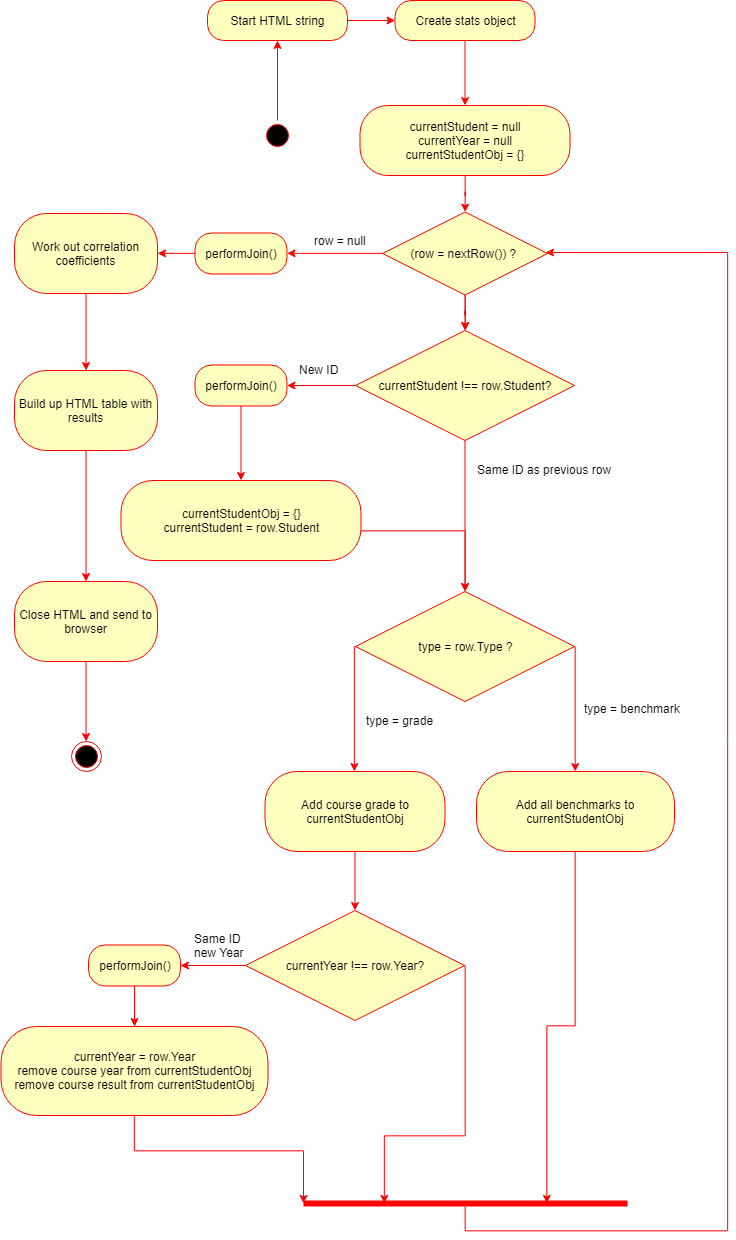
\includegraphics[scale=0.5]{./resources/figures/fig-listfn-correlation-grades.png}
    \end{mdframed}
    \caption[\textit{List}-function: \texorpdfstring{grades $\bowtie$ admissions}{Lg}]{\textbf{Figure \ref{fig-listfn-correlation-grades}: \textit{List}-function: \texorpdfstring{grades $\bowtie$ admissions}{Lg}}}
    \label{fig-listfn-correlation-grades}
\end{figure}

\begin{table}[H]
    \begin{threeparttable}
        \textbf{Table \ref{tbl-correlation-grades}}\par\medskip\par\medskip
        \caption{Correlation between different benchmarking methods and CSC1015F grades}
        \label{tbl-correlation-grades}
        \begin{tabularx}{\textwidth}{>{\hsize=1.3\hsize}X>{\hsize=0.7\hsize}Y}
            \toprule
            \mC{c}{Benchmark}                     & \mC{c}{$r$} \\
            \midrule
            Gr12 Eng \%                           & 0.287       \\
            Gr12 Sci \%                           & 0.465       \\
            Gr12 Mth \%                           & 0.447       \\
            NBT AL \%                             & 0.368       \\
            NBT QL \%                             & 0.533       \\
            NBT Mth \%                            & 0.510       \\
            Avg Gr12 \%                           & 0.485       \\
            Avg Gr12 \% (Dbl Mth)                 & 0.487       \\
            Avg Gr12 \% (Dbl Mth \& Sci)          & 0.493       \\
            Avg NBT \%                            & 0.583       \\
            Avg NBT \% (Dbl AL)                   & 0.559       \\
            Avg NBT \% (Dbl QL)                   & 0.580       \\
            Avg NBT \% (Dbl Mth)                  & 0.583       \\
            Avg NBT \% (Dbl AL/QL)                & 0.567       \\
            Avg NBT \% (Dbl AL/Mth)               & 0.570       \\
            Avg NBT \% (Dbl QL/Mth)               & 0.589       \\
            Avg Gr12 \& NBT                       & 0.610       \\
            Avg Gr12 \& NBT (Dbl Gr12 Mth)        & 0.587       \\
            Avg Gr12 \& NBT (Dbl Gr12 Mth \& Sci) & 0.578       \\
            \bottomrule
        \end{tabularx}
    \end{threeparttable}
\end{table}